\chapter{体感系统的受体} \label{chap:chap18}

神经生理学对个体感觉方式的研究首先在体感系统中进行,该系统传输由分布在全身的受体编码信息。
\textit{查尔斯$\cdot$谢林顿}是最早研究这些身体感觉的人之一,他指出体感系统具有 3 个主要功能:本体感觉、外感觉和内感觉。


本体感觉是自己的感觉。
骨骼肌、关节囊和皮肤中的受体使我们能够有意识地感知到自己身体的姿势和运动,尤其是四肢和头部。
尽管可以在没有\textit{本体感受器}感觉反馈的情况下移动身体的某些部分,但这些运动往往笨拙、协调性差,并且不能充分适应复杂的任务,尤其是在缺乏视觉指导的情况下。


外部感受是在影响身体时与外部世界直接互动的感觉。
外部感受的主要模式是触觉,包括接触、压力、抚摸、运动和振动的感觉,用于识别物体。
一些触觉涉及主动运动组件(抚摸、敲击、抓握或按压)由此身体的一部分相对于另一个表面或生物体移动。
在大脑中,触觉的感觉和运动部分在解剖学上是紧密相连的,对指导行为很重要。


外部感觉还包括热感觉和冷感觉。
热感觉是行为和\textit{内稳态}机制的重要控制者,需要保持体温接近37°C。
最后,外部感受包括疼痛感或伤害感受,是对损害或伤害身体的外部事件响应。
伤害感受是生存所必需行动的主要动机,例如战斗或逃跑。


躯体感觉的第 3 个组成部分(内感受)是身体主要器官系统的功能及其内部状态的感觉。
内脏受体传递的信息对于调节自主功能至关重要,特别是在心血管、呼吸、消化和肾脏系统中,尽管这些受体记录的大多数刺激不会导致有意识的感觉。
中间受体主要是通过血气和酸碱值等指标监测器官功能的化学受体,以及感知组织膨胀(可能被认为是疼痛)的机械受体。


这组不同的感觉功能似乎不太可能组合形成 1 个感觉系统。
我们在介绍性章节中介绍了所有躯体感觉,因为它们是由一类感觉神经元,即\textit{背根神经节}神经元介导的。
来自皮肤、肌肉、关节囊和内脏的体感信息由支配四肢和躯干的\textit{背根神经节}神经元或支配颅骨结构(面部、嘴唇、口腔、结膜和硬脑膜)的三叉感觉神经元传递。
这些感觉神经元执行 2 个主要功能:
将刺激转导和编码为电信号,以及将这些信号传输到中枢神经系统。


在过去的 10 年里,躯体感觉的研究因 3 项重要进展而发生了革命性的变化。
首先,开发具有\textit{背根神经节}神经元基因表达荧光报告基因的转基因小鼠,使神经科学家能够评估特定受体类别的生理响应及其对身体和中枢神经系统中感觉受体的解剖预测。
表达基因编码的钙传感器(如\textit{钙瞬变的遗传标记}6)的单个\textit{背根神经节}神经元的功能成像可以同时光学记录支配身体特定区域的受体神经元群的活动,从而为分析对体感刺激的整体响应提供有用的工具。
其次,在体外对分离的\textit{背根神经节}神经元或在减少的皮肤神经制剂中进行研究,可以对受体响应进行生物物理评估,并对单个体感神经元中表达的离子通道进行表征。
第三,将压电蛋白离子通道鉴定为哺乳动物机械受体中触觉和本体感觉的分子传感器,为评估这些通道在触觉、本体感觉和内脏功能中的作用提供了一个新的系统。


在本章中,我们将考虑所有\textit{背根神经节}神经元的共同原理以及区分它们各自感觉功能的原理。
我们首先描述周围神经及其组织,然后调查负责每种主要身体感觉的受体类别。
我们还研究了将各种刺激能量转化为电信号的感觉传导机制。
然后,我们描述了父轴突在其感受野中整合来自多个受体的信息,最后讨论了脊髓和脑干中每个亚模态的中央处理中心。
触觉、疼痛、本体感觉和内脏自主调节的高阶处理将在后面的章节中描述。



\section{背根神经节神经元是体感系统的初级感觉受体细胞}

\textit{背根神经节}神经元的细胞体位于脊神经或脑神经背根的神经节中。
背根神经节神经元起源于神经嵴,与附近的脊髓节段密切相关。
\textit{背根神经节}中的单个神经元由于其外围末端的形态学和分子特化而选择性地响应特定类型的刺激。


背根神经节神经元是一种双极细胞,称为伪单极细胞。 
如图~\ref{fig:18_1}~所示,\textit{背根神经节}神经元的轴突有 2 个分支,1 个投射到外周,1 个投射到中枢神经系统。
单个\textit{背根神经节}神经元的外周末梢支配皮肤、肌肉、关节囊或内脏,并包含专门用于特定种类刺激的受体。 
如图~\ref{fig:18_13}~所示,受这些感觉末梢支配的身体区域称为皮节。
感觉周围神经末梢在受体形态和刺激选择性方面有所不同,使它们能够检测机械、热或化学事件。
中央分支终止于脊髓或脑干,形成体感通路中的第一个突触。
因此,每个\textit{背根神经节}细胞的轴突作为单一传输线,在受体末端和中枢神经系统之间具有一个极性。
该轴突称为初级传入纤维。


\begin{figure}[htbp]
	\centering
	\includegraphics[width=0.65\linewidth]{chap18/fig_18_1}
	\caption{背根神经节的神经元是体感系统的初级感觉细胞。
		细胞体位于与脊髓相邻的\textit{背根神经节}中。
		轴突有 2 个分支,一个投射到身体,其专用末端包含特定形式刺激能量的受体,另一个投射到脊髓或脑干,传入信号在这里被处理。
		所有\textit{背根神经节}神经元都包含 5 个功能区:
		1. 皮肤、肌肉或内脏的远末端包含专门的受体通道,可将特定类型的刺激能量(机械、热或化学)转化为去极化受体电位。
		\textit{背根神经节}神经元通常具有多个感觉末梢。
		2. 脉冲生成位点包含电压门控的~\ce{Na+} 通道和~\ce{K+} 通道(Na$_\text{V}$ 和 K$_\text{V}$),它们位于受体囊内轴突起始段附近;它们将受体电位转化为动作电位流。
		3. 周围神经纤维将动作电位从棘突起始部位传递到背根神经节细胞体。 
		4. \textit{背根神经节}神经元的细胞体包含在与脊髓或脑干相邻的神经节内。 
		5. 脊神经或脑神经将\textit{背根神经节}或三叉神经元连接到同侧脊髓或脑干。}
	\label{fig:18_1}
\end{figure}


支配身体特定区域(例如拇指或手指)的单个初级传入纤维聚集在一起,形成周围神经的轴突束或束。
它们在发育过程中被各种营养因子引导到体内的特定位置,例如\textit{脑源神经营养因子}、\textit{神经营养因子} 3、\textit{神经营养因子} 4或\textit{神经生长因子}。
外周神经还包括支配附近肌肉、血管、腺体或内脏的运动轴突。


周围神经或其大脑靶点的损伤可能会导致特定肌肉群中不止一种体感亚模式或运动缺陷的感觉缺陷。
了解体感模式在形态学上的重叠位置和分叉位置,有助于神经系统疾病和功能障碍的诊断。


如图~\ref{fig:18_1}~所示,每个\textit{背根神经节}神经元可细分为 5 个功能区:感受区、脉冲生成部位、周围神经纤维、\textit{背根神经节}细胞体、脊髓或脑神经。
如图~\ref{fig:3_9}A~所示,位于\textit{背根神经节}轴突远端的感受区包含专门的受体蛋白,它能感知局部环境中的机械力、热事件或化学物质,并将这些信号转化为轴突末梢的局部去极化,称为受体电位。
如图~\ref{fig:3_10}A~所示,这种局部去极化被动地向产生动作电位的中央轴突扩散,通常在初始段(远端到有髓纤维中\textit{郎飞结}的第一个节点)。
足够强度的刺激会产生动作电位,这些动作电位沿着周围神经纤维传递,通过细胞体,并进入终止于脊髓或脑干的中央分支。


\textit{背根神经节}神经元的躯体包含细胞核。 
感觉受体蛋白在体细胞中表达,为体外表征它们的电导特性提供了一个方便的表达系统。 
分离的\textit{背根神经节}神经元已广泛用于感觉受体电流和电压门控动作电位通道的膜片钳研究。


\textit{背根神经节}神经元在细胞体大小、基因表达谱、轴突传导速度、感觉转导分子、体内神经支配模式和生理功能方面存在差异。
例如,如图~\ref{fig:18_2}~所示,支配感觉触觉和本体感觉的机械受体的\textit{背根神经节}具有最大的细胞体和大的有髓轴突;
它们表达 \textit{神经肽Y受体2} 或\textit{小清蛋白}等蛋白质。
相比之下,如图~\ref{fig:18_2}C、D~所示,感知温度或刺激性化学物质的\textit{背根神经节}神经元具有小细胞体和无髓鞘轴突;
它们表达\textit{降钙素基因相关肽}或\textit{植物凝集素}。
当这些荧光分子标记通过轴突延伸到它们在身体和中枢神经系统中的外周末梢时,\textit{大卫$\cdot$金蒂}及其同事能够表征身体中体感神经末梢的模式(图~\ref{fig:18_2}H)并追踪它们的中枢投射到脊髓(图~\ref{fig:18_2}G)和脑干。

\begin{figure}[htbp]
	\centering
	\includegraphics[width=1.0\linewidth]{chap18/fig_18_2}
	\caption{背根神经节神经元的大小、基因表达和皮肤神经支配模式各不相同\cite{li2011functional}。
		图 A-F 显示通过胸背根神经节对组织切片进行双重免疫染色。
		这些部分中的单个\textit{背根神经节}神经元表达特定类别的体感神经纤维的遗传标记。
		G 蛋白偶联受体 \textit{神经肽Y受体2}-\textit{绿色荧光蛋白}(绿色)或 \textit{神经肽Y受体2}-TOM(红色)在生理学上标记了 A$\beta$ 快适应低阈值机械受体(A$\beta$ \textit{快适应}-\textit{低阈值机械受体})。
		这些纤维还表达\textit{神经丝重多肽},这是重度髓鞘轴突(E)的标志物,形成纵向披针形(梳状)末端,围绕着毛茸茸的皮肤中的单个针毛或锥子/紫红色毛发(H),并终止于层板 III 到 V 的背角(G)。 
		双标神经元或纤维被染成黄色。
		A. A$\beta$ \textit{快适应}-\textit{低阈值机械受体}在发育早期表达受体酪氨酸激酶\textit{转染重排}(命名为早期 \textit{转染重排}并染成红色)。
		大多数这些神经元也表达 \textit{神经肽Y受体2}-\textit{绿色荧光蛋白}(绿色);
		表达这 2 种标记的神经元被染成黄色。 A$\beta$ \textit{快适应}-\textit{低阈值机械受体}具有中等大小的细胞体。
		B. A$\beta$ \textit{快适应}-\textit{低阈值机械受体}(绿色)比\textit{本体感受器}(例如肌梭传入神经和表达小白蛋白的高尔基肌腱器官)具有更小的细胞体(\textit{小清蛋白},红色)。
		C、D. A$\beta$ \textit{快适应}-\textit{低阈值机械受体}(\textit{神经肽Y受体2}-\textit{绿色荧光蛋白},绿色)比释放\textit{三磷酸腺苷}作为共递质(\textit{植物凝集素},红色)的无髓鞘嘌呤 C 纤维和表达\textit{降钙素基因相关肽}(红色)的肽能 A$\delta$ \textit{低阈值机械受体}具有更大的细胞体 。
		E. 具有大细胞体的重度髓鞘周围神经纤维表达\textit{神经丝重多肽}(绿色)。
		这些包括\textit{大直径}和 Ib 组肌肉传入神经、A$\beta$ SA-\textit{低阈值机械受体} 和 A$\beta$ \textit{快适应}-\textit{低阈值机械受体}(也标有 \textit{神经肽Y受体2}-tdTom [红色])。
		只有 A$\beta$ \textit{快适应}-\textit{低阈值机械受体} 表达这 2 种标记并被染成黄色。
		F-H. 用 \textit{神经肽Y受体2}-\textit{绿色荧光蛋白}(绿色)和 \textit{神经肽Y受体2}-\textit{红色荧光蛋白}(红色)对胸部\textit{背根神经节}神经元(F)、它们在脊髓背角版板 III 至 V 层中地中央突起(G),以及它们在毛发皮肤切片中毛囊处的外周披针形末端(H)进行双重免疫染色,结果显示标记的外周和中央 A$\beta$ \textit{快适应}-\textit{低阈值机械受体} 神经元在很大程度上彼此重叠(黄色),并且此类遗传标记可用于追踪感觉神经末梢。}
	\label{fig:18_2}
\end{figure}



\section{周围体感神经纤维以不同的速率传导动作电位}

将脉冲序列从脉冲产生部位传输到中枢神经系统的外周神经通常用作体感受体机制的神经生理学研究的主要记录部位。
动物的单个周围神经纤维通常从主轴突束中分离出来,并放置在用作记录电极的细线上。
微电极(由锋利的钨丝或铂丝制成)也已通过皮肤插入人体周围神经(一种称为显微神经造影术的技术),以测量对各种躯体刺激的感觉响应(第~\ref{chap:chap19}~章)。


周围神经纤维根据与轴突直径和髓鞘形成、传导速度以及它们是感觉神经纤维还是运动神经纤维的相关特性,被分为功能组。
第一个神经分类方案由\textit{查尔斯$\cdot$谢林顿}于 1894 年设计,他测量了感觉神经中髓磷脂染色的轴突的直径,随后由\textit{大卫$\cdot$劳埃德}编纂(表~\ref{tab:18_1})。
如图~\ref{fig:18_3}~所示,他们发现了 2 个或 3 个重叠的轴突直径组。
后来发现这些解剖学分组在功能上很重要。
肌肉神经中的 I 组轴突支配肌梭受体和高尔基肌腱器官,它们发出肌肉长度和收缩力的信号。
II 组纤维支配关节囊中的次级纺锤体末梢和受体;
这些受体还介导本体感觉。
第 III 组纤维、最小的有髓鞘肌肉传入神经,和无髓鞘的第 IV 组传入神经发出感觉为疼痛的肌肉和关节外伤或损伤信号。


\begin{table}[htbp]
	\caption{外周神经感觉纤维的分类} \label{tab:18_1} \centering
	\begin{tabular}{lllll}
		\toprule
		 & 肌肉神经 & 皮神经 & 纤维直径(微米) & 传导速度(米/秒)\\
		\midrule
		\textit{有髓鞘} &  &  & &  \\
		大直径 & I  & A$\alpha$ & 12–20 & 72–120 \\
		中直径 & II  & A$\beta$ & 6–12 & 36–72 \\
		小直径 & III  & A$\delta$ & 1–6 & 4–36 \\
		无髓鞘 & IV  & C & 0.2–1.5 & 0.4–2.0 \\
		\bottomrule
	\end{tabular}
\end{table}



\begin{figure}[htbp]
	\centering
	\includegraphics[width=0.6\linewidth]{chap18/fig_18_3}
	\caption{哺乳动物外周神经纤维的分类。
	直方图显示了支配骨骼肌和皮肤的 4 组感觉神经纤维的轴突直径分布。
	每组都有一个特征性的轴突直径和传导速度(见表~\ref{tab:18_1})。
	浅蓝色线标记重叠区域中每组光纤轮廓的边界。
	有髓外周神经纤维的传导速度(米/秒)约为纤维直径(微米)的 6 倍。}
	\label{fig:18_3}
\end{figure}



支配皮肤的神经包含 2 组有髓神经纤维:
II 类纤维支配对触觉有响应的皮肤机械受体,III 类纤维介导热刺激和伤害性刺激,以及多毛皮肤中的轻触。
无髓鞘的第 IV 组皮肤传入神经与肌肉中的神经传入神经一样,也可介导热刺激和有害刺激。


另一种对周围神经纤维进行分类的方法是基于对整个神经的电刺激。
在这种广泛使用的诊断技术中,神经传导速度在放置在周围神经上方皮肤上的成对刺激电极和记录电极之间测量。
例如,在研究\textit{正中神经}或\textit{尺神经}的传导时,可以将刺激电极放置在手腕上,将记录电极放置在上臂上。
通过刺激电极施加的短暂电脉冲在神经中引起动作电位。
短时间后在手臂中记录的神经信号代表了刺激脉冲激发的所有神经纤维的动作电位总和,称为复合动作电位(第~\ref{chap:chap9}~章)。
随着更多的神经纤维受到刺激,它的振幅会增加;
总的活动大致与活动神经纤维的总数成正比。


如图~\ref{fig:18_4}~所示,强度增加的电刺激首先在最大的轴突中诱发动作电位,因为它们具有最低的电阻,然后逐渐在较小的轴突中诱发动作电位。
大直径纤维传导动作电位的速度更快,因为电流沿轴突流动的内阻较低,而且\textit{郎飞结}沿其长度分布较宽(第~\ref{chap:chap9}~章)。
大有髓纤维的传导速度(以米/秒为单位)大约是轴突直径(以微米为单位)的 6 倍,而细有髓纤维的传导速度是轴突直径的 5 倍。
对于无髓纤维,将轴突直径转换为传导速度的系数为 1.5 至 2.5。


\begin{figure}[htbp]
	\centering
	\includegraphics[width=1.0\linewidth]{chap18/fig_18_4}
	\caption{临床上通过复合动作电位测量周围神经的传导速度。
		不同强度的周围神经电刺激会激活不同类型的神经纤维。
		由特定电流量刺激的所有神经的动作电位相加以产生复合动作电位。
		不同类别的感觉和运动轴突的不同传导速度产生多个峰值\cite{erlanger2016electrical}。}
	\label{fig:18_4}
\end{figure}


在刺激伪影之后,复合动作电位中记录的最早神经信号出现在传导速度大于 90 米每秒的纤维中。
如图~\ref{fig:18_4}~所示,该信号被称为 A$\alpha$ 波,反映了 I 组纤维和支配骨骼肌的运动神经元中产生的动作电位。
在受神经支配的区域中,受试者几乎无法感知到这种感觉。


随着更多大纤维被募集,出现第二个信号,即 A$\beta$ 波。
该成分对应于皮肤或肌肉神经中的 II 组纤维,这些神经支配调节触觉和本体感觉的机械受体,并且随着电击强度的增加而变大。
在较高的电压下,当较小的 A$\delta$ 范围内的轴突被募集时,刺激会变得疼痛,类似于静电产生的电击。
足以激活无髓鞘 C 纤维的电压会引起灼痛感。
正如我们将在本章后面了解到的那样,一些 A$\delta$ 和 C 纤维也会对毛茸茸的皮肤上的轻触做出响应,但是当整个神经受到电刺激时,这种温和的触觉刺激会被同时激活的痛觉纤维所掩盖。
如图~\ref{fig:18_9}~所示,刺激支配肌梭梭内纤维的运动神经元会引发称为 A$\gamma$ 波的中间小波,但这通常很难辨别,因为这些运动神经元的传导速度与 A$\beta$ 和 A$\delta$ 感觉轴突的传导速度重叠。
这些周围神经纤维直径和传导速度的差异使得触觉和本体感觉信号比有害或热信号更早到达脊髓和更高的大脑中枢。


\begin{figure}[htbp]
	\centering
	\includegraphics[width=1.0\linewidth]{chap18/fig_18_9}
	\caption{肌梭是本体感觉的主要受体。
		A. 肌梭位于骨骼肌内,在肌肉伸展时兴奋。
		它由一对感觉轴突缠绕的一束细(梭内)肌纤维组成。
		它也受几个运动轴突(未显示)支配,这些运动轴突产生梭内肌纤维的收缩。
		感觉神经末梢中的拉伸敏感离子通道通过蛋白质血影蛋白与细胞骨架相连\cite{sachs1992stretch}。
		B. 支配肌梭的\textit{大直径组纤维}中记录的去极化受体电位与平行于肌丝的肌肉拉伸的速度和幅度成正比。
		当拉伸保持在固定长度时,受体电位会衰减到较低的值\cite{cone1971transducer}。
		C. 肌细胞中单个拉伸敏感通道的膜片钳记录。
		通过吸力对受体细胞膜施加压力。
		静止时(0 厘米汞柱),通道会在短时间间隔内偶尔打开。 
		随着施加到膜上的压力增加,通道打开得更频繁并且保持打开状态的时间更长。
		这允许更多的电流流入受体细胞,从而导致更高水平的去极化\cite{guharay1984stretch}。}
	\label{fig:18_9}
\end{figure}


临床医生利用各种传入纤维的传导速度已知分布来诊断导致感觉纤维退化或运动神经元丢失的疾病。
在某些情况下,周围神经轴突的丢失是选择性的;
例如,在糖尿病的神经病变特征中,大直径感觉纤维退化。
这种选择性丧失反映在复合动作电位适当峰值的减少、神经传导的减慢以及相应的感觉能力的减弱上。
同样,在多发性硬化症中,中枢神经系统中大直径传入纤维的髓鞘退化会导致神经传导减慢,如果足够严重,还会导致神经传导失败。


\section{体感系统使用多种特殊受体}

单个\textit{背根神经节}神经元的功能特化由发生在身体远端神经末梢的感觉转导的分子机制决定。
当躯体受体被适当的刺激激活时,其感觉末端通常是去极化的。
如图~\ref{fig:3_9}~A~所示,去极化的幅度和时间进程反映了刺激的强度及其持续时间。
足够强度的刺激会产生动作电位,这些动作电位会沿着\textit{背根神经节}神经元轴突的外周分支传递到终止于脊髓或脑干的中央分支。


介导触觉和本体感觉的感觉神经元终止于非神经囊(图~\ref{fig:18_1})或在毛囊(图~\ref{fig:18_2} H)或梭内肌纤维(见图~\ref{fig:18_9}A)周围形成形态上独特的末端。
它们感觉到机械刺激会缩进或拉伸他们的感受面。
相比之下,检测有害、热或化学事件的神经元外周轴突具有带多个分支的无鞘末端,这些分支终止于表皮或内脏。


几种不同的形态学特化受体是各种体感亚模式的基础。
例如,支配手部皮肤的正中神经和一些控制手部的肌肉包含数以万计的神经纤维,可分为 30 种功能类型。
其中,22 种类型是传入纤维(感觉轴突将冲动传导至脊髓),8 种类型是传出纤维(运动轴突将冲动从脊髓传导至骨骼肌、血管和汗腺)。
传入纤维传递来自对不同类型的皮肤变形敏感的 8 种皮肤机械受体的信号;
5 种\textit{本体感受器}发出有关肌肉力量、肌肉长度和关节角度的信息;
报告接触皮肤的物体温度的 4 种温度受体;
以及 4 种发出潜在伤害性刺激信号的伤害受体。
表~\ref{tab:18_2}~中列出了每个子模态中的主要受体组。


\begin{table}[htbp]
	\caption{在躯体感觉加工中活跃的受体类型} \label{tab:18_2} \centering
	\begin{tabular}{llllll}
		\toprule
		受体类型 & 纤维组 & 纤维名称 & 受体 & 标记 & 模态\\
		\midrule
		\textit{皮肤机械受体} & &  &  &  & 触摸 \\
		梅克尔盘受体 & A$\alpha$、$\beta$ & \textit{慢适应}1\textit{型} & \makecell[l]{压电型机械敏感\\离子通道组件}2 & \makecell[l]{Troma1/\\Keratin8/\\\textit{神经肽Y受体2}} & \makecell[l]{压力、\\纹理} \\
		环层小体 & A$\alpha$、$\beta$ & RA2 & \makecell[l]{压电型机械敏感\\离子通道组件}2 & \makecell[l]{cRet/\\\textit{神经肽Y受体2}/\\\textit{神经丝重多肽}} & 振动 \\
		鲁菲尼终末器 & A$\alpha$、$\beta$ & SA2 & \makecell[l]{压电型机械敏感\\离子通道组件}2 &  & 皮肤拉伸 \\
		毛发(保护) & A$\alpha$、$\beta$ & A$\beta$ \textit{快适应}-LTMR & \makecell[l]{压电型机械敏感\\离子通道组件}2 & \makecell[l]{cRet/\\\textit{神经肽Y受体2}/\\神经丝重多肽} & 毛发运动 \\
		\makecell[l]{毛发(awl\\/auchene)} & A$\delta$ & \makecell[l]{A$\delta$-\\LTMR} & \makecell[l]{压电型机械敏感\\离子通道组件}2 & TrkB & 轻抚、吹气 \\
		\makecell[l]{域受体(\\圆周端)} & \makecell[l]{A$\beta$(\\Field\\-LTMR)} & A$\beta$ & \makecell[l]{压电型机械敏感\\离子通道组件}2 & \textit{神经丝重多肽} & 皮肤拉伸 \\
		毛发(锯齿形) & C & C-LTMR &  & TH & \makecell[l]{慢抚、轻柔\\的触碰} \\
		温度受体 &  &  &  &  & 温度 \\
		冷受体 & A$\delta$ & III & \textit{瞬时受体电位}M\textit{型}8 &  & \makecell[l]{皮肤冷却\\(小于 25°C)} \\
		热受体 & C & IV & \makecell[l]{瞬时受体电位\\香草醛受体3} &  & \makecell[l]{皮肤变暖\\(高于 35°C)} \\
		热伤害受体 & A$\delta$ & III & \makecell[l]{瞬时受体电位\\香草醛受体1\\瞬时受体电位\\香草醛受体2} &  & 高温(高于 45°C) \\
		冷伤害受体 & C & IV & \makecell[l]{瞬时受体电位\\\textit{锚定蛋白}1\\瞬时受体电位\\M型8} &  & 低温(低于 5°C) \\
		\textit{疼痛受体} &  &  & &  & 疼痛 \\
		机械 & A$\delta$ & III & & \makecell{降钙素基因\\相关肽} & \makecell[l]{锐利的\\东西、刺痛} \\
		热机械(热) & A$\delta$ & III & \makecell[l]{瞬时受体电位\\香草醛受体2} &  & 灼痛 \\
		热机械(冷) & C & IV & \makecell[l]{瞬时受体电位\\香草醛受体1\\瞬时受体电位\\textit{锚定蛋白}1} & \textit{植物凝集素} & 冷痛 \\
		多觉型 & C & IV & \makecell[l]{瞬时受体电位\\香草醛受体1/\\瞬时受体电位\\textit{锚定蛋白}1} &  & \makecell[l]{缓慢、灼热\\的疼痛} \\
		\textit{肌肉和骨骼} &  &  &  &  & 肢体本体感觉 \\
		\textit{机械受体} &  &  &  &  &  \\
		肌梭原发性 & A$\alpha$ & 大直径 & \makecell[l]{压电型机械敏感\\离子通道组件}2 & PV/NFH & \makecell[l]{肌肉长度\\和速度} \\
		肌梭继发 & A$\beta$ & II & \makecell[l]{压电型机械敏感\\离子通道组件}2 & PV/NFH & 肌肉伸展 \\
		高尔基腱器官 & A$\alpha$ & Ib & \makecell[l]{压电型机械敏感\\离子通道组件}2 & PV/NFH & 肌肉收缩 \\
		关节囊受体 & A$\beta$ & II &  &  & 关节角度 \\
		伸缩敏感自由端 & A$\delta$ & III &  &  & \makecell[l]{过度拉伸\\或用力} \\
		\bottomrule
	\end{tabular}
\end{table}


\subsection{机械受体介导触觉和本体感受}

机械受体感知周围组织的物理变形。
机械扩张(例如皮肤压力、肌肉拉伸、直接作用于细胞膜的吸力或组织的渗透性肿胀)通过刺激细胞膜中机械受体离子通道的物理作用转化为电能。
如图~\ref{fig:3_9}A~所示,机械刺激使受体蛋白变形,从而打开拉伸敏感离子通道,并增加使受体神经元去极化的非特异性阳离子电导。
去除刺激可以缓解受体上的机械应力,并允许拉伸敏感通道关闭。


已经提出机械受体离子通道激活的各种机制。
如图~\ref{fig:18_5}A~所示,一些机械受体似乎对通过细胞质膜脂质的张力或变形传递的力作出响应,这种机制称为来自脂质的力。
在这里,膜脂的变形改变了细胞表面的曲率,将受体蛋白中的疏水残基暴露给膜磷脂,从而打开通道孔以供阳离子流动。
这可能是检测细胞肿胀的机制,它在渗透压调节或由于流体流动改变引起的血管壁剪切应力变化中起着重要作用。


\begin{figure}[htbp]
	\centering
	\includegraphics[width=0.7\linewidth]{chap18/fig_18_5}
	\caption{机械受体神经末梢中的离子通道被拉伸或变形细胞膜的机械刺激激活。
		机械位移导致通道打开,允许阳离子流入\cite{lin2005trp}。
		A. 来自脂质的力。
		通道可以被通过细胞膜中脂质张力传递的力直接激活,例如血压的变化。
		B. 来自细丝的力。
		通过连接到离子通道的结构蛋白传递的力也可以直接激活机械感觉通道。
		连接结构蛋白可以是细胞外的(附着在周围组织上)或细胞内的(与细胞骨架结合)或两者兼而有之。}
	\label{fig:18_5}
\end{figure}


如图~\ref{fig:18_5}B~所示,机械受体激活的另一种假定机制涉及通过结构蛋白将通道蛋白连接到周围组织,这种机制称为细丝作用力。
在这种排列中,通过组织的直接压力或横向拉伸施加到皮肤或肌肉的机械力会扭曲细胞外基质或细胞内细胞骨架蛋白(肌动蛋白、整合素、微管)。
这些束缚分子与受体通道蛋白相互作用,改变它们的构象,并打开阳离子通道。
与通道蛋白的细胞外连接是有弹性的,通常表示为弹簧门。
该模型中的直接通道门控可能由拉伸细胞外连接蛋白的力产生。
当力被移除时,通道关闭。
这种类型的直接通道门控被内耳的毛细胞和皮肤中的一些触觉受体使用。


值得注意的是,虽然\textit{埃德加$\cdot$阿德里安}和\textit{左特曼}在 1920 年代首先研究了皮肤触觉的受体末端器官,并且在 1960 年代从肠系膜(\textit{环层小体})分离的触觉受体记录了受体电位,但关于哺乳动物触摸中机械感觉的分子生物学几乎没有达成共识 。
领先的候选者来自无脊椎动物模型生物(例如线虫秀丽隐杆线虫),其触觉受体被确定为离子通道变性蛋白超家族的成员,类似于脊椎动物上皮~\ce{Na+}通道(\textit{退化蛋白}/\textit{上皮钠离子通道})。
其他候选分子包括\textit{瞬时受体电位香草醛受体}4(也参与热感觉的瞬时受体电位 [\textit{瞬时受体电位}] 受体的成员)和\textit{无机械感受器电位C},\textit{瞬时受体电位}N 家族的果蝇成员。
然而,这些分子不在哺乳动物\textit{背根神经节}神经元中表达。


跨膜离子通道的压电蛋白家族最近被\textit{雅顿$\cdot$帕塔普蒂安}及其同事鉴定为哺乳动物机械感受的分子介质。
如图~\ref{fig:18_6}A~所示,\textit{压电型机械敏感离子通道组件}1蛋白由大约 2,500 个氨基酸组成,至少有 26 个跨膜 $\alpha$ 螺旋。
离子通道是由 3 个相同的 \textit{压电型机械敏感离子通道组件} 蛋白亚基形成的三聚体,每个\textit{压电型机械敏感离子通道组件}蛋白的 C 末端有 2 个成孔 $\alpha$ 螺旋。
如图~\ref{fig:18_6}B~所示,亚基的 N 端形成螺旋桨状结构,这被认为与耦合机械刺激与通道门控有关。
压电蛋白形成非特异性阳离子可渗透通道,可传导兴奋性去极化电流。


\begin{figure}[htbp]
	\centering
	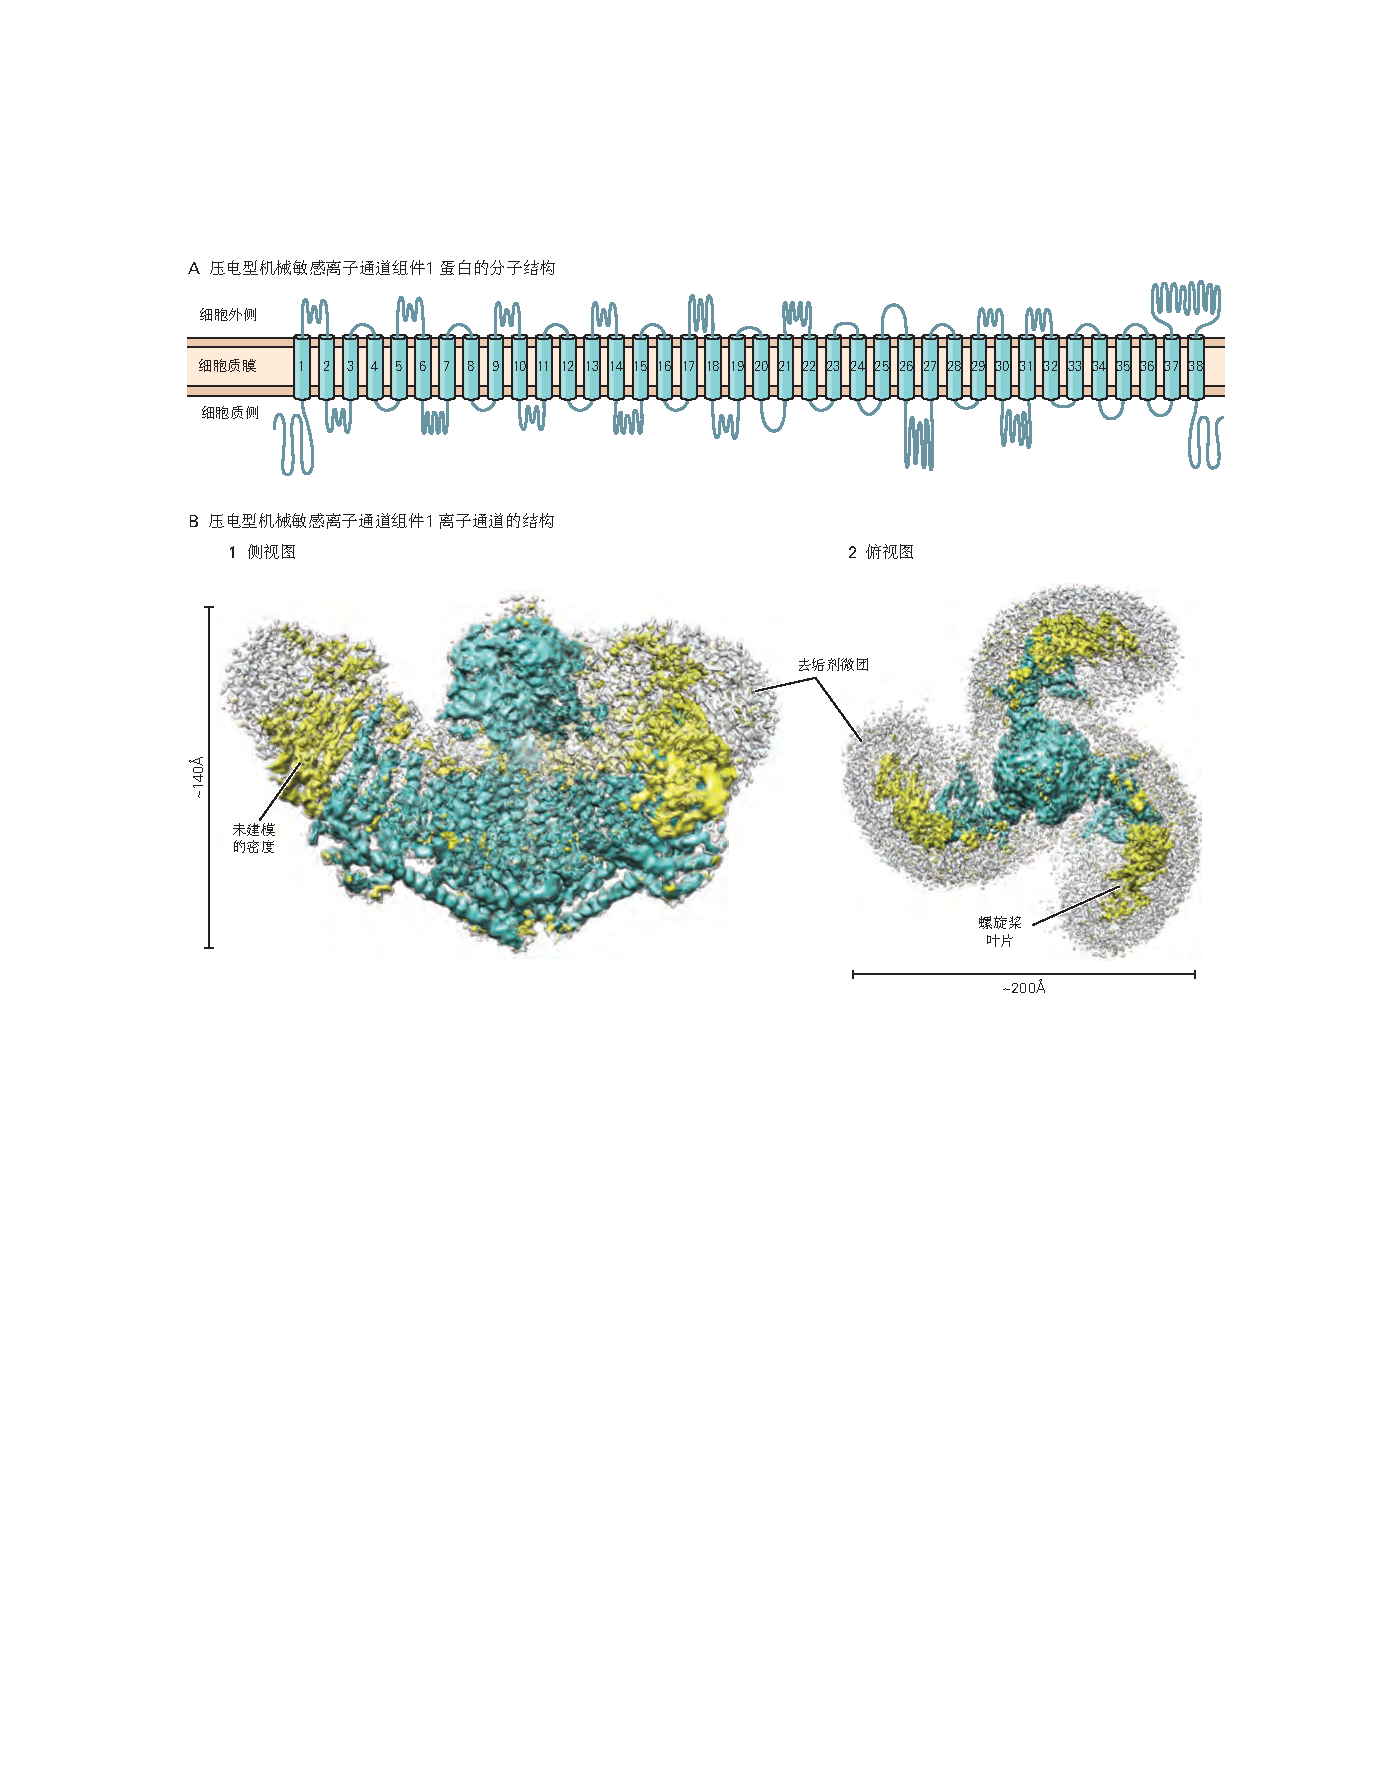
\includegraphics[width=1.0\linewidth]{chap18/fig_18_6}
	\caption{\textit{压电型机械敏感离子通道组件}1离子通道的结构和分子组织。
		A. \textit{压电型机械敏感离子通道组件}1和\textit{压电型机械敏感离子通道组件}2具有同源蛋白质结构,包含大约 2,500 个氨基酸,至少有 26 个假定的跨膜片段。
		它们组合成三聚体,形成哺乳动物体内最大的膜离子通道\cite{murthy2017piezos}。
		B. 从低温电子显微镜推断出的\textit{压电型机械敏感离子通道组件}1离子通道的推定结构。
		1. 侧面观,胞浆面朝下。
		2. 从细胞外侧俯视图。
		受体是由 3 个相同的\textit{压电型机械敏感离子通道组件}1亚基组成的三脚架。
		3 种压电蛋白的 C 端形成一个中央细胞外帽,连接到跨膜孔的细胞外表面,跨膜孔延伸到膜外进入细胞质尾区。
		穿过通道的水孔延伸穿过帽的中心轴、跨膜孔和细胞质尾区。
		3 个蛋白质亚基的N-末端排列在外围,形成螺旋桨状的螺旋结构。
		蓝色表示高分辨率建模区域\cite{saotome2018structure}。}
	\label{fig:18_6}
\end{figure}



\textit{压电型机械敏感离子通道组件}蛋白的 2 种不同亚型用作机械传感器:
\textit{压电型机械敏感离子通道组件}1主要存在于非神经组织中,例如血管、肾脏和膀胱中的上皮细胞,以及红细胞。
\textit{压电型机械敏感离子通道组件}2 在调节触觉和本体感觉的机械感觉\textit{背根神经节}和三叉神经神经元中表达,在支配肺部平滑肌的迷走神经传入神经中表达,它们通过感知肺部伸展来调节\textit{肺牵张反射}(第~\ref{chap:chap32}~章)。



\subsection{专门的末梢器官有助于机械感觉}

除了在远端神经末梢表达的离子通道分子组成外,周围组织的成分(如上皮细胞或肌纤维),在机械传导中也起着重要作用。
围绕\textit{背根神经节}神经元神经末梢的特殊非神经终末器官必须以特定方式变形以激发纤维。
例如,个体机械受体选择性地响应压力或运动,从而检测施加到皮肤、关节或肌肉纤维力的方向。
末端器官还可以放大或调节受体轴突对机械位移的敏感性。


皮肤中的特殊上皮细胞(例如\textit{梅克尔细胞}、毛囊内衬的上皮细胞和形成无毛皮肤指纹的乳头状脊)在触觉中起着重要的辅助作用。
这些末端器官中研究得最好的是\textit{梅克尔细胞}(感觉上皮细胞),在表皮-真皮交界处与大直径(A$\beta$)感觉神经轴突的末梢形成紧密接触,形成\textit{梅克尔细胞}-神经突复合物。
\textit{梅克尔细胞}聚集在多毛皮肤表皮的肿胀处,称为触摸圆顶(图~\ref{fig:18_7}A),在无毛皮肤中靠近指纹脊的中心(见图~\ref{fig:19_3})。
如图~\ref{fig:18_7}A2~所示,当探头接触触摸圆顶时,感觉神经会响应一系列动作电位,其频率与施加到皮肤上压力的速度和幅度成正比。
这些脉冲序列通常在整个刺激期间持续,并被称为慢适应(因为放电持续长达 30 分钟)。
同样,感觉神经称为\textit{慢适应}1\textit{型}纤维。


\begin{figure}[htbp]
	\centering
	\includegraphics[width=1.0\linewidth]{chap18/fig_18_7}
	\caption{支配\textit{梅克尔细胞}的传入纤维对皮肤上的压力不断做出响应。
		A. 1. 一个\textit{慢适应}1\textit{型}机械感受纤维支配多毛皮肤触摸圆顶中的 22 个\textit{梅克尔细胞}簇(每个细胞都标有\textit{增强型绿色荧光蛋白})。
		左图:分离的皮肤神经记录制剂的体内荧光图像。
		星号(*)表示相关防护毛发在触摸球内的位置。
		右图:由\textit{慢适应}1\textit{型}纤维支配的整个触控圆顶的共聚焦 z 系列投射。
		箭头用于对齐 2 个图像中的\textit{梅克尔细胞}。
		2. \textit{慢适应}1\textit{型}纤维响应施加在触摸圆顶(上部记录)上的 5 秒持续时间步长的压力(以\textit{千帕}为单位),具有不规则的、缓慢适应的脉冲序列(在细胞外记录),其平均\textit{激活率}和施加的力(较低的记录)成正比 。
		神经元在刺激开始时以最高速率发射,而在维持压力期间发射较少的脉冲。
		B. \textit{慢适应}1\textit{型}机械受体中的感觉转导模型。
		皮肤上的压力会打开\textit{梅克尔细胞}中的 \textit{压电型机械敏感离子通道组件}2 通道(蓝色)以及接收来自\textit{梅克尔细胞}的突触输入的\textit{慢适应}1\textit{型}纤维的外周神经突。
		神经突中的 \textit{压电型机械敏感离子通道组件}2 通道在刺激(1)开始时打开,产生对触摸的初始动态响应(2)。
		皮肤变形同时激活\textit{梅克尔细胞}(3)中的 \textit{压电型机械敏感离子通道组件}2 通道,使其去极化并允许\textit{梅克尔细胞}(4)中的电压门控 Ca$_V$ 通道持续打开和释放神经递质(5)。
		神经递质的结合进一步使\textit{慢适应}1\textit{型}轴突去极化,从而在主轴突中产生持续放电(6)\cite{maksimovic2014epidermal}。}
	\label{fig:18_7}
\end{figure}


\textit{梅克尔细胞}在触觉方面的感受功能类似于耳蜗中的听觉毛细胞(第~\ref{chap:chap26}~章)和舌头中的味觉细胞(第~\ref{chap:chap32}~章)。
体外研究的\textit{梅克尔细胞}对压力或吸力等机械力作出响应,去极化电流在时间过程和电导方面与孤立的\textit{背根神经节}神经元中诱发的电流相似。
它们表达突触释放蛋白并包含在持续压力下释放兴奋性神经递质的囊泡。
\textit{梅克尔细胞}表达 \textit{压电型机械敏感离子通道组件}2 蛋白,并在压力刺激下显示细胞质 \ce{Ca^2+} 水平升高。


\textit{梅克尔细胞}对触觉生理响应的重要性在未能在表皮中形成\textit{梅克尔细胞}的小鼠(Atoh1 条件性基因敲除小鼠)中可见。
与野生型相比,这些动物中\textit{慢适应}1\textit{型}纤维的放电率在振幅和持续时间上有所降低。
这些实验表明\textit{梅克尔细胞}负责对静态触摸的持续响应。
最近,如图~\ref{fig:18_7}B~所示,\textit{艾伦$\cdot$伦普金}及其同事使用\textit{梅克尔细胞}的光遗传学刺激而不是直接对皮肤施加压力来证明支配触摸圆顶的\textit{慢适应}1\textit{型}纤维使用双重机制来感知皮肤上的压力。
对触摸的初始动态响应主要由流过\textit{慢适应}1\textit{型}神经末梢 \textit{压电型机械敏感离子通道组件}2 通道的电流产生。
随后的静态响应由\textit{梅克尔细胞}的兴奋性突触传递引起,\textit{梅克尔细胞}表达 \textit{压电型机械敏感离子通道组件}2 通道并在持续对皮肤施加压力时不断释放神经递质。


从皮肤表面突出的毛发提供了另一组重要的触摸端器官。 
感觉毛发纤维对运动极其敏感。
微风或吹气使头发偏转会从毛囊传入纤维中激发一种或多种动作电位。
人类可以感知单根毛发的运动,并将这种感觉定位于毛发根部,也就是毛发从皮肤中露出来的地方。
感觉毛发具有重要的保护功能,因为它们会在物体、其他生物体或环境中的障碍物影响身体之前检测到它们。
毛发或感觉触角检测重要的物体特征(如纹理、曲率和刚度),这些特征有助于识别朋友或敌人。
这些神经元被命名为\textit{快适应低阈值机械受体},因为当头发受到外力移动时,它们会对轻柔的触摸或头发运动做出短暂的脉冲响应。


头发嵌入称为毛囊的皮肤内陷中。
如图~\ref{fig:18_8}A~所示,在哺乳动物皮肤中发现了 3 种类型的毛发。
最大、最长和最硬的毛发(称为针毛)在发育过程中最先从皮肤长出。
针毛由直径最大、传导速度最快的感觉神经纤维(A$\beta$ 型)支配;
如图~\ref{fig:18_2}H~所示,这些纤维在毛发周围的毛囊表皮形成披针形(梳状)末端。
A$\beta$ \textit{快适应}-\textit{低阈值机械受体} 神经纤维还支配具有披针形末梢的中等大小的毛发(称为锥形毛/桃红毛)。
Awl/auchene 毛发具有三重神经支配:
它们为快速传导(A$\beta$)有髓纤维提供输入;
直径更小、传导速度更慢的有髓(A$\delta$)纤维;
和无髓鞘的 C 纤维。
最小和最多的毛发(称为之字形或绒毛)也受 A$\delta$ 和 C 纤维支配。


\begin{figure}[htbp]
	\centering
	\includegraphics[width=1.0\linewidth]{chap18/fig_18_8}
	\caption{低阈值机械受体对多毛皮肤的神经支配。
		A. 哺乳动物的多毛皮肤受\textit{低阈值机械受体}的特定组合支配;
		这些多类神经纤维允许触摸信息沿着多条并行神经纤维传输到中枢神经系统。
		\textit{梅克尔细胞}的触摸圆顶位于大直径保护毛周围的表皮-真皮边界。
		\textit{梅克尔细胞}的轴突被归类为 A$\beta$ \textit{慢适应}1\textit{型}-\textit{低阈值机械受体},它们约占支配多毛皮肤的感觉纤维的 3\%。
		保护毛囊由快适应的触觉纤维支配,分类为 A$\beta$ \textit{快适应}-\textit{低阈值机械受体},在毛囊周围形成纵向披针形(梳状)末端。
		它们构成了另外 3\% 的支配多毛皮肤的感觉纤维。
		A$\beta$ \textit{快适应}-\textit{低阈值机械受体} 纤维还在中等大小的锥形/紫红色毛发上形成披针形末端; 每根纤维支配邻近皮肤区域的多个毛囊。
		Awl/auchene 毛发由 3 种不同类别的感觉纤维的披针形末端支配;
		A$\beta$ \textit{快适应}-\textit{低阈值机械受体}(蓝色)、A$\delta$-\textit{低阈值机械受体}(红色,7\% 的纤维)和 C-\textit{低阈值机械受体}(绿色,15\%–27\% 的纤维)。
		锯齿形或绒毛是数量最多的类型;
		它们受直径最小、传导速度最慢的周围神经纤维(A$\delta$- C-\textit{低阈值机械受体})支配。 
		所有 3 种类型的毛囊也由圆周末端(黄色)支配\cite{zimmerman2014gentle}。
		B. 整个皮肤切片说明\textit{低阈值机械受体}感觉神经末梢在多毛皮肤和可激活单个感觉纤维皮肤区域中的扩散。
		所有 5 个类别都支配多个毛囊并具有分支的感觉神经末梢。
		比例尺(适用于所有图像)= 500 微米。 
		这些轴突中的每一个的放电率都反映了来自皮肤中多个受体末端器官的输入。
		A$\beta$-\textit{低阈值机械受体}在所有类别的毛囊周围形成圆周末端;
		它们在毛茸茸的皮肤中拥有最大的感受野,支配多达 180 个毛囊/纤维,跨越面积达 6 平方毫米。
		A$\beta$ \textit{慢适应}1\textit{型}-\textit{低阈值机械受体}具有最小的感受野,但支配触摸圆顶内的所有\textit{梅克尔细胞};
		每个触控圆顶仅由 1 个 A$\beta$ \textit{慢适应}1\textit{型}-\textit{低阈值机械受体}支配。
		A$\beta$ \textit{快适应}- A$\delta$-\textit{低阈值机械受体} 和 C-\textit{低阈值机械受体}形成披针形末端,包围多达 40 个单独的毛囊,跨越 0.5 至 4 平方毫米的皮肤区域\cite{bai2015genetic}。}
	\label{fig:18_8}
\end{figure}


直到最近,A$\delta$ 和 C 纤维还被认为只调节热觉或痛觉。
然而,\textit{约翰$\cdot$威斯伯格}、\textit{哈肯$\cdot$奥劳森}和\textit{亚克$\cdot$威尔波}对人类进行的显微神经造影研究表明:毛茸茸的皮肤也受到无髓鞘 C-\textit{低阈值机械受体} 纤维的支配,这些纤维对缓慢移动的触觉刺激做出响应,并被认为可以调节社交或愉悦的触觉。
它们还可能在脊髓背角的疼痛抑制中发挥作用。


皮肤中毛囊的神经支配模式说明了身体感觉神经支配的 2 个重要原则:汇聚和发散。
皮肤中的每个毛囊都为多种感觉传入纤维提供输入。
这种重叠模式提供了一小块皮肤的感觉输入冗余。
共享的通信线路支配每个毛囊,而不是单一的标记线路。 
因此,来自皮肤的触觉信息由一组感觉神经元并行传输。


由\textit{背根神经节}神经元的感觉神经末梢支配的皮肤区域定义了细胞的感受野,即可以激发细胞的身体区域。
每条感觉神经纤维都从广泛的皮肤区域收集信息,因为它的远端末梢有多个可以独立激活的分支。
这种形态使每条传入纤维能够为大脑提供独特的感觉输入模式。


图~\ref{fig:18_8}B~说明了不同类别的\textit{背根神经节}神经元所包含的感受野大小和区域的多样性。
由于触觉感受野的面积很大,轻柔的触摸会在接触部位激发许多不同的感觉纤维,每一种都传达一种特定的感觉信息。
最小的触觉感受野是由\textit{慢适应}1\textit{型}纤维支配的触摸圆顶(参见图~\ref{fig:19_8}B A$\beta$ \textit{慢适应}1\textit{型})。
单个\textit{慢适应}1\textit{型}纤维支配触摸圆顶中的所有\textit{梅克尔细胞},通常从相邻皮肤区域的 1 到 3 个触摸圆顶收集信息。
如图~\ref{fig:19_8}B A$\beta$ \textit{快适应}~所示,由单个\textit{快适应}纤维支配的毛囊分布得更远,感觉末梢的大小略有不同,直径最大的 A$\beta$ 纤维包含最小的毛囊感受野。
皮肤中最大的感受野是 A$\beta$ 场受体(参见图~\ref{fig:19_8}B A$\beta$ 场)。
这些纤维在毛囊周围形成圆周末端,但对毛发运动或吹气没有响应。
取而代之的是,场受体会在其感受区内对抚摸皮肤或拉伸皮肤做出响应。
场受体也会因拉扯头发或强压力等疼痛刺激而兴奋,这表明它们也可能介导机械疼痛的感觉。



\subsection{\textit{本体感受器}测量肌肉活动和关节位置}

肌肉和关节中的机械受体传达有关身体姿势和运动的信息,从而在本体感觉和运动控制中发挥重要作用。
感觉神经末梢与骨骼肌、肌腱、关节囊和皮肤的机械耦合被认为是本体感觉的基础。
这些受体包括 2 种类型的肌肉长度传感器,即\textit{大直径}型和 II 型肌梭末梢;
一个肌肉力传感器,高尔基肌腱器官;
关节囊受体,可传导关节囊中的张力;
和感觉皮肤在关节上伸展的\textit{鲁菲尼终末器}。


如图~\ref{fig:18_9}A~所示,肌梭由一束细肌纤维或梭内纤维组成,它们与较大的肌肉纤维平行排列并封闭在胶囊内。
由于神经末梢中的机械感受性离子通道,梭内纤维被一对感觉轴突缠绕在一起,这些轴突检测肌肉拉伸。
梭内肌还接收来自调节收缩力和受体敏感性的运动轴突的输入(有关肌梭的详细信息,请参见文本框~\ref{box:32_1})。


如图~\ref{fig:18_9}B~所示,尽管肌梭传入纤维的受体电位和放电率与肌肉长度成正比,但这些响应可以通过大脑中调节梭内肌肉收缩的更高中枢来调节。
因此,纺锤体传入纤维能够对内部产生\textit{自主运动}的幅度和速度以及外力造成的被动肢体位移进行编码(第~\ref{chap:chap32}~章)。


位于骨骼肌和肌腱交界处的高尔基肌腱器官测量肌肉收缩产生的力(有关高尔基肌腱器官的详细信息,请参见文本框~\ref{box:32_4})。
尽管这些受体在调节肌肉力量的反射回路中起着重要作用,但它们似乎对肌肉活动的有意识感觉贡献不大。
肌肉疲劳或部分瘫痪的心理物理学实验表明,感知的肌肉力量主要与集中产生的力量有关,而不是与实际肌肉力量有关。


\textit{雅顿$\cdot$帕塔普蒂安}及其同事最近的研究表明:\textit{压电型机械敏感离子通道组件}2 介导来自肌梭和高尔基肌腱器官的传入纤维传输的信号,因为这些纤维在其远端和细胞体中表达 \textit{压电型机械敏感离子通道组件}2 蛋白。


关节受体在关节角度的姿势感觉中几乎没有作用。
相反,对近端关节(例如肘部或膝盖)角度的感知取决于来自肌梭受体的传入信号和传出运动命令。
此外,手指位置和手形的有意识感觉取决于皮肤牵张受体和肌梭。



\subsection{热受体检测皮肤温度的变化}

虽然手持物体的大小、形状和质地可以通过视觉和触觉来理解,但物体的热特性是独一无二的体感。
人类识别 4 种不同类型的热感觉:冷、凉、暖和热。
这些感觉由大约 32°C 的正常皮肤温度与空气或接触身体的物体的外部温度之间的差异引起。
与疼痛和瘙痒的其他原发病方式一样,温度感由多种受体类型的组合编码介导,由小直径传入纤维传递。


虽然人类对皮肤温度的突然变化非常敏感,但我们通常不会意识到皮肤温度的大幅波动,这由于我们的皮肤血管扩张或收缩以释放或保存体温而发生。
如果体表温度变化缓慢,我们不会意识到 31° 至 36°C 范围内的变化。
在 31°C 以下,感觉从凉爽发展为寒冷,最后在 10° 至 15°C 时开始发展为疼痛。
高于 36°C 时,感觉会从温暖变为热,然后从 45°C 开始变为疼痛。


热感觉由表皮中的游离神经末梢介导。
这些神经纤维信号的温度范围由小直径\textit{背根神经节}神经元的远端神经末梢和细胞体中表达的受体分子的分子组成决定。
如图~\ref{fig:18_10}~所示,\textit{大卫$\cdot$朱利斯}及其同事的研究表明,热刺激会激活这些神经元中特定类别的\textit{瞬时受体电位}通道。
\textit{瞬时受体电位}通道由与产生动作电位的电压门控通道属于同一基因超家族的基因编码(第~\ref{chap:chap8}~章)。 
它们形成介导内向去极化电流的非选择性阳离子通道。
\textit{瞬时受体电位}通道包含 4 个相同的蛋白质亚基,每个亚基包含 6 个跨膜 $\alpha$-螺旋,在第五和第六螺旋之间有一个成孔元件。
单个\textit{瞬时受体电位}受体的区别在于它们对热或冷的敏感性,当超过其热阈值时,显示出对阳离子的电导率急剧增加。
它们的名称指定了\textit{瞬时受体电位}受体的遗传亚家族和成员编号。 
示例包括\textit{瞬时受体电位香草醛受体}1、\textit{瞬时受体电位}M\textit{型}8和\textit{瞬时受体电位锚定蛋白}1。



\begin{figure}[htbp]
	\centering
	\includegraphics[width=1.0\linewidth]{chap18/fig_18_10}
	\caption{瞬时受体电位离子通道。
		\textit{瞬时受体电位}通道由具有 6 个跨膜 $\alpha$-螺旋的膜蛋白组成。
		在 4 个亚基的第 5 个(S5)和第 6 个(S6)螺旋之间形成 1 个孔。
		大多数这些受体在 N 末端结构域中包含\textit{锚定蛋白}重复序列,在 C 末端结构域中包含与 S6 相邻的常见 25 氨基酸基序。
		单个\textit{瞬时受体电位}通道由 4 个相同的\textit{瞬时受体电位}蛋白组成。
		所有\textit{瞬时受体电位}通道都由温度和各种化学配体门控,但不同类型对不同温度范围有响应并具有不同的激活阈值。
		在感觉神经元中至少鉴定出 6 种类型的\textit{瞬时受体电位}受体; 神经元的热敏感性由其神经末梢表达的特定\textit{瞬时受体电位}受体决定。
		在 32°C 的静息皮肤温度(星号)下,只有 \textit{瞬时受体电位香草醛受体}4 和一些 \textit{瞬时受体电位香草醛受体}3 受体受到刺激。
		\textit{瞬时受体电位锚定蛋白}1 和\textit{瞬时受体电位}M\textit{型}8 受体被冷却和冷刺激激活。
		\textit{瞬时受体电位}M\textit{型}8 受体也对薄荷醇和各种薄荷有响应;
		\textit{瞬时受体电位锚定蛋白}1 受体对大蒜和萝卜等表达葱的植物有响应。
		\textit{瞬时受体电位香草醛受体}3 受体被温暖的刺激激活并结合樟脑。
		\textit{瞬时受体电位香草醛受体}1 和 \textit{瞬时受体电位香草醛受体}2 受体对热有响应并产生灼痛感。 
		\textit{瞬时受体电位香草醛受体}1 通道还对可引起疼痛的各种物质、温度或力作出响应。
		它们对受体的作用位点包括辣椒活性成分(辣椒素)、酸(柠檬汁)、蜘蛛毒液的结合位点,以及第二信使激活激酶的磷酸化位点。
		\textit{瞬时受体电位香草醛受体}4 受体在正常皮肤温度下是活跃的并且对触摸有响应\cite{jordt2003lessons}。}
	\label{fig:18_10}
\end{figure}


两类\textit{瞬时受体电位}受体在寒冷温度下激活,在升温时被灭活。
\textit{瞬时受体电位}M\textit{型}8 受体对低于 25°C 的温度有响应(这样的温度被认为是凉爽或寒冷的)。
\textit{瞬时受体电位锚定蛋白}1 受体的热阈值低于 17°C ;
这个范围被描述为寒冷或极冷。
\textit{瞬时受体电位}M\textit{型}8和\textit{瞬时受体电位锚定蛋白}1受体均在高阈值冷受体末端表达,但只有\textit{瞬时受体电位}M\textit{型}8受体在低阈值冷受体末端表达。


来自低阈值冷受体的热信号通过表皮内具有无髓末端的小直径有髓鞘 A$\delta$ 纤维传输。
这些纤维表达瞬时受体电位通道 \textit{瞬时受体电位}M\textit{型}8 并对应用于皮肤的薄荷醇作出响应。
冷受体对皮肤温度突然下降的敏感度大约是对逐渐变化敏感度的 100 倍。
这种对变化的极端敏感性使人类能够从远处打开的窗户检测到气流。


4 种类型的\textit{瞬时受体电位}受体被温暖或高温激活,在冷却时失活。
\textit{瞬时受体电位香草醛受体}3 在暖型纤维中表达;
它们对高于 35°C 的皮肤升温做出响应,并产生从暖到热的各种感觉。
\textit{瞬时受体电位香草醛受体}1 和 \textit{瞬时受体电位香草醛受体}2 对超过 45°C 的温度有响应并介导灼痛感;
它们在热伤害受体中表达。 
\textit{瞬时受体电位香草醛受体}4 受体在 27°C 以上的温度下活跃,并发出正常皮肤温度的信号。


暖受体位于终止于真皮的 C 纤维末端。
与冷受体不同,暖受体更像是简单的温度计。
它们的放电率随着皮肤温度的升高而单调上升,直至达到疼痛阈值,然后在更高的温度下达到饱和。
与冷受体相比,暖受体对皮肤温度的快速变化不太敏感。
因此,人类对变暖的响应不如对冷却的响应;
即使是最敏感的受试者,检测皮肤突然变暖的阈值变化也约为 0.1°C。


热伤害受体在超过 45°C 的温度下被激活,并在皮肤冷却时失活。
高温引起的灼痛由有髓 A$\delta$ 纤维和无髓 C 纤维共同传递。


\textit{瞬时受体电位}受体在热感觉中的作用最初通过分析辣椒素和薄荷醇等天然物质发现,这些物质在应用于皮肤或皮下注射时会产生灼烧感或凉爽感。
辣椒素是辣椒中的活性成分,已被广泛用于激活伤害性 C 纤维传入神经,介导灼痛感。
这些研究表明,各种\textit{瞬时受体电位}受体还结合其他分子,这些分子会引起疼痛感,例如毒素、毒液以及患病或受伤组织释放的物质。
\textit{瞬时受体电位锚定蛋白}1 受体结合辛辣物质,例如辣根(芥末)、大蒜、洋葱和类似的葱属植物。
这些物质表现为刺激物,可能通过共价修饰 \textit{瞬时受体电位锚定蛋白}1 蛋白中的半胱氨酸而产生疼痛或瘙痒。


如图~\ref{fig:20_2}~所示,\textit{瞬时受体电位}通道是多模态感觉整合器,因为蛋白质的不同部分直接响应温度、pH 值或渗透压的变化;
存在有毒物质,例如辣椒素或毒素;
或被细胞内第二信使磷酸化。
第~\ref{chap:chap20}~章详细介绍了它们的分子结构和在疼痛中的作用。



\subsection{伤害受体介导疼痛}

对可能损伤组织的刺激有选择性响应的受体称为伤害受体。
它们直接对机械和热刺激作出响应,并通过受伤组织中细胞释放的化学物质间接对其他刺激作出响应。
伤害受体发出即将发生的组织损伤信号,更重要的是,它们不断提醒组织已经受伤,必须加以保护。


疾病或创伤导致的主要器官系统功能异常会引起有意识的疼痛感。
我们对疼痛神经机制的大部分了解都来自对皮肤伤害受体的研究,因为在皮肤神经中研究这些机制比在内脏神经中更容易研究。
然而,内脏痛的神经机制与身体表面疼痛的神经机制相似。


皮肤、肌肉、关节和内脏受体中的伤害受体根据其传入纤维的髓鞘形成分为 2 大类。
由薄髓鞘 A$\delta$ 纤维支配的伤害受体产生短延迟疼痛,被描述为尖锐和刺痛。
大多数被称为机械伤害受体或\textit{高阈值机械受体},因为被尖锐物体穿透、挤压或挤压皮肤(图~\ref{fig:18_11})或通过拉动多毛皮肤中的毛发而兴奋。
许多这些纤维还会对 45°C 以上的温度产生响应,从而灼伤皮肤;
这些 A$\delta$ 纤维还表达热敏 \textit{瞬时受体电位香草醛受体}2 通道。


\begin{figure}[htbp]
	\centering
	\includegraphics[width=0.9\linewidth]{chap18/fig_18_11}
	\caption{机械伤害受体会对刺破、挤压或捏住皮肤的刺激做出响应。
		刺激皮肤中具有游离神经末梢的 A$\delta$ 纤维会产生尖锐的刺痛感。
		这些受体对刺破皮肤的尖锐物体有响应(B),但对来自钝头探针的强大压力没有响应(A)。
		最强的响应是用锯齿钳夹住皮肤产生的,这会损坏接触区域的组织(C)\cite{perl1968myelinated}。}
	\label{fig:18_11}
\end{figure}


受 C 纤维支配的伤害受体会产生弥漫性局限性且难以耐受的钝痛、灼痛。
最常见的类型包括多模态伤害受体,它们对各种有害的机械、热和化学刺激做出响应,例如捏或刺、有害的热和冷,以及应用于皮肤的刺激性化学物质。
如第~\ref{chap:chap20}~章所述,大多数 C 多觉型伤害受体表达 \textit{瞬时受体电位香草醛受体}1 和/或\textit{瞬时受体电位锚定蛋白}1 受体。
人体对这些纤维的电刺激会引起长时间的灼痛感。
在内脏中,伤害受体被膨胀或肿胀激活,产生剧烈疼痛感。


\subsection{痒是一种独特的皮肤感觉}

痒是一种常见的感觉体验,局限于皮肤、眼结膜和粘膜。 
它与疼痛有一些共同的特性,直到最近,它还被认为由伤害感受纤维的低放电率引起。
就像疼痛一样,无论其强度如何,瘙痒本质上都是令人不快的。
即使以引起疼痛为代价,我们也试图通过抓挠来消除它。


\textit{戴安娜$\cdot$保蒂斯塔}和\textit{莎拉$\cdot$威尔逊}最近的研究表明:表达\textit{瞬时受体电位香草醛受体}1 和 \textit{瞬时受体电位锚定蛋白}1 受体的 C 纤维介导由瘙痒(产生瘙痒)剂诱发的瘙痒感。
由皮内注射组胺或通过释放内源性组胺的程序引起的瘙痒会激活一部分表达 \textit{瞬时受体电位香草醛受体}1 的神经元,这些神经元也含有 H1 组胺受体;
这些瘙痒感会被抗组胺药阻断。
组胺非依赖性瘙痒似乎由表达 \textit{瞬时受体电位锚定蛋白}1 通道的 C 纤维\textit{背根神经节}介导。
该通路中的瘙痒感是由皮肤干燥或与\textit{Mas相关G蛋白偶联受体}家族成员结合的瘙痒原触发的,例如抗疟药氯喹。


当\textit{瞬时受体电位锚定蛋白}1 受体还参与感知有害的寒冷温度(低于 15°C)时,它们如何调节瘙痒?
为什么一些表达 \textit{瞬时受体电位香草醛受体}1 的纤维介导瘙痒感而不是热毒感?
答案在于小直径感觉神经纤维对组合编码的使用。
例如,当\textit{瞬时受体电位锚定蛋白}1 和 \textit{瞬时受体电位}M\textit{型}8 受体都处于兴奋状态时,会感觉到有害的寒冷,而当 \textit{瞬时受体电位}M\textit{型}8 受体处于沉默状态时,会感觉到瘙痒。
同样,当表达 \textit{瞬时受体电位香草醛受体}1、\textit{瞬时受体电位香草醛受体}2 和 \textit{瞬时受体电位香草醛受体}3 的纤维被共同激活时,会感觉到热痛,但当只有表达 \textit{瞬时受体电位香草醛受体}1 的纤维有响应而 \textit{瞬时受体电位香草醛受体}2 和 \textit{瞬时受体电位香草醛受体}3 受体处于沉默状态时,可能会感觉到痒。
使用多个受体的类似组合编码通常被其他化学感官(例如嗅觉和味觉)使用。



\subsection{内脏感觉代表五脏六腑的状态}

本能感觉很重要,因为它们驱动对生存至关重要的行为,例如呼吸、进食、饮水和繁殖。
前面描述的用于研究背根神经节和三叉神经节中的触觉、疼痛、热感觉和本体感觉的相同分子遗传策略已被用于对迷走神经感觉神经节中的内脏传入进行分类。
\textit{斯蒂芬$\cdot$利伯莱斯}及其同事最近分析了迷走神经感觉神经节(结节/颈静脉复合体)中的感觉响应,该神经节接收来自肺、心血管、免疫或消化系统的机械感觉或化学感觉信息。


迷走神经传入纤维表达多种\textit{G-蛋白偶联受体},这些受体已用荧光抗体标记,以识别其在特定内脏中的外周感觉受体位点,并标记其在延髓孤束核特定区域的独特中心投射。
通过在已识别的迷走神经节神经元中表达\textit{钙瞬变的遗传标记},\textit{利伯莱斯}及其同事测量了它们对机械刺激的生理响应,例如拉伸或它们被营养素或胃激素(5-羟色胺、胰高血糖素样肽 1 或胆囊收缩素)激活。
标记特定迷走神经传入的能力为分析内脏功能的神经调节和追踪用于调节这些重要身体功能的通路提供了重要工具。


尽管它们的细胞体似乎随机散布在迷走神经核中,但单个迷走神经元在特定器官系统中执行不同的感觉功能。
例如,对已识别的迷走神经感觉神经元进行光遗传学刺激表明:至少有 2 个控制呼吸的迷走神经元群。
表达\textit{G-蛋白偶联受体} \textit{嘌呤能受体P2Y1} 的神经元会诱发呼吸暂停,在呼气时将肺困住,而表达\textit{G-蛋白偶联受体} \textit{神经肽Y受体2} 的神经元会产生快速浅呼吸。
刺激这些神经元对心率或消化功能没有影响。
另一组\textit{G-蛋白偶联受体}用于标记调节胃肠功能的神经元。
一组胃传入是感知胃和上肠扩张并调节胃动力的机械受体,而其他胃传入是感知肠道中特定营养素并帮助其吸收的化学受体。



\section{动作电位编码将体感信息传递给大脑}

在前面的部分中,我们了解到各种刺激,如机械力、温度和各种化学物质,与\textit{背根神经节}神经元远端轴突末梢的受体分子相互作用,产生感觉末梢的局部去极化。
如第~\ref{chap:chap17}~章所述,这些受体电位被转换为动作电位的数字脉冲编码,以传输到中枢神经系统。


周围神经纤维的感觉末端区域通常是无髓鞘的,并且不表达构成动作电位生成基础的电压门控~\ce{Na+} 通道和~\ce{K+} 通道。
例如,如图~\ref{fig:18_2}H~所示,毛囊传入的披针形末端是无髓鞘的。
这种设计通过将高度分支的末端膜区域专用于感觉转导通道(例如 \textit{压电型机械敏感离子通道组件}2 或\textit{瞬时受体电位}受体)来优化感受野中的信息收集。


如图~\ref{fig:3_10}~所示,有髓纤维中最远端的动作电位离子通道通常位于初始髓鞘段附近或无髓纤维中分支的交叉点。
这对信息传输具有重要影响。
如果参与动作电位生成的通道不存在于接受终端,则来自多个分支的去极化感觉信号可以更容易地累加,因为动作电位的再生特性和电压门控 \ce{Na+} 通道随后的失活。
来自后激活受体的感觉信息可能会因与沿纤维另一分支传播的向后传播动作电位的碰撞而消失。
因此,沿着初级传入轴突传输的信号可能是感官刺激的非线性反射,反映了来自多个分支的激发的空间总和或对后期产生活动的赢者通吃抑制。
不同神经突分支的顺序激活还可以通过生成长串动作电位来帮助检测移动刺激,前提是个体末梢以最佳速率受到刺激,这样它们的响应就不会被其他分支中较早产生的脉冲分流。



沿周围神经的动作电位传递取决于轴突是有髓鞘还是无髓鞘以及每根神经纤维中电压门控~Na$_\text{V}$ 和 K$_\text{V}$ 通道的特定亚类的表达。
\textit{史蒂文$\cdot$韦克斯曼}及其同事报告说,支配\textit{本体感受器}和\textit{低阈值机械受体}的大直径 A$\alpha$ 和 A$\beta$ 纤维主要表达 Na$_\text{V}$1.1 和 Na$_\text{V}$1.6 亚型;
这些纤维通常以高速率激发动作电位,部分原因是它们还表达能够使轴突快速复极化的 K$_\text{V}$1.1 通道和 K$_\text{V}$1.2 通道。
介导痛痒感觉的小直径外周神经表达 Na$_\text{V}$1.7 通道、Na$_\text{V}$1.8 通道和 Na$_\text{V}$1.9 通道。
后 2 种 Na$_\text{V}$ 亚型具有促进重复放电的动力学和电压敏感性,从而增强疼痛感:
Na$_\text{V}$ 1.8 通道在动作电位期间不完全失活并在它们之后迅速恢复; 
Na$_\text{V}$ 1.9 通道在相对负电位下激活并经历可忽略不计的失活,导致持续的内向电流可以放大亚阈值刺激。



\subsection{感觉神经节提供了群体对躯体刺激的响应快照}

我们通过检查单个哺乳动物体感神经节内感觉响应的分布来结束对\textit{背根神经节}神经元的研究。
通常,一次研究一个周围神经纤维,通常对特定受体类别进行最佳刺激。
然而,即使是微弱的声音也会对神经合唱产生影响,而经典的单细胞记录技术在很大程度上忽略了这些声音。


新的体内功能成像技术为标记、可视化和测量对各种类型体感刺激的整体响应提供了有用的工具。
例如,由感觉刺激诱发的 \ce{Ca^2+} 电流提供了单个神经元脉冲序列电生理记录的替代方法。
在图~\ref{fig:18_12}~所示的实验中,基因编码的 \ce{Ca^2+} 传感器\textit{钙瞬变的遗传标记}6f 在小鼠三叉神经节细胞中表达,该神经节还表达多觉型 \textit{瞬时受体电位香草醛受体}1,使研究人员能够可视化和量化由各种神经元激活的神经元群的活动。
\textit{尼姆$\cdot$基塔尼}、\textit{亚历山大$\cdot$切斯勒}及其同事使用\textit{威廉$\cdot$威利斯}首先开发的一系列触觉刺激、有害刺激和热刺激来分析脊髓神经元的体感响应,同时记录了 213 个三叉神经元的响应\cite{2017Specialized}。
他们的发现非常了不起。
如~\ref{fig:18_12}B1~的热力图所示,神经元响应多种多样,对相同刺激的放电模式强度和持续时间差异很大。
这种整体记录技术表明:即使在受体水平上,也没有对躯体刺激的规范响应,而是常见的响应模式。

\begin{figure}[htbp]
	\centering
	\includegraphics[width=0.85\linewidth]{chap18/fig_18_12}
	\caption{支配面部多毛皮肤的三叉神经节神经元的体感模式分布\cite{ghitani2017specialized}。
		A. 表达 \textit{瞬时受体电位香草醛受体}1-\textit{钙瞬变的遗传标记}6f 的小鼠中三叉神经节进行体内荧光成像。
		钙敏感染料(\textit{钙瞬变的遗传标记}6f)响应 \ce{Ca^2+} 通过电压门控通道进入单个三叉神经节神经元而发出荧光。
		A1. 小鼠三叉神经节中 213 个表达 \textit{钙瞬变的遗传标记}6f 的神经元的解剖位置。
		比例尺为 500 微米。
		这些神经元广泛分布在三叉神经节内。 
		A2. 对大于 40°C 的热脉冲或对头发拉动有响应的神经元子集中~\ce{Ca^2+}信号的高倍放大图像;
		左图中的颜色条表示每个神经元中~\ce{Ca^2+} 信号的强度。
		最强的活动以白色或红色显示;
		蓝色响应最弱。
		比例尺为 100 微米。
		A3. 以伪彩色标记的 2 个群体映射的叠加(红色代表热,绿色代表头发拉扯)显示哪些神经元对每个刺激有响应。
		这些神经元通常对热或头发拉动有选择性,但有 2 个对 2 种方式都有响应(黄色)。
		B. 量化在该三叉神经节中可视化的所有表达 \textit{瞬时受体电位香草醛受体}1 的神经元对各种触觉、有害和热刺激模式的响应。
		B1. 同时记录的所有 213 个标记神经元对抚摸脸颊、有害机械(拉头发)和热刺激的响应的热力图。
		每行说明了单个神经元对这些刺激的响应;
		像素颜色表示每个神经元响应的强度(Δf/F)(颜色范围 = 10\%–60\% Δf/F)。
		神经元响应按放电率增加的时间开始垂直排序。
		热力图上方的符号表示刺激的类型和顺序:
		顺着毛发或逆着毛发生长的方向抚摸脸颊、拉毛,以及范围从 25°C 到 47°C 到 12°C 的热刺激。
		尽管这些神经元中有一半以上对轻柔的触摸(抚摸)有响应,但它们通常对有害的机械刺激(头发拉动)的响应比对抚摸皮肤的响应更强烈。
		观察到对有害热的最强响应,但此类神经元仅占所研究群体的 30\%。
		在实验结束时,来自每个神经元的记录被分类到 B2 中确定的 7 个响应类别之一。
		B2. 7 类三叉神经感觉响应的 \ce{Ca^2+} 信号平均响应幅度和时间过程。
		注意使用这种客观的神经元分类模式响应的多模态性质。
		B3. 饼图说明了每个类别中神经元的数量和比例。}
	\label{fig:18_12}
\end{figure}


此外,个体体感神经元似乎是多感觉的,对不止一种方式做出响应,例如触摸和疼痛。
如图~\ref{fig:18_12}A~所示,这项研究表明:个体三叉神经元可以区分有害热和机械性疼痛(头发拉扯),并且可以对轻柔的触摸或适度的热刺激做出响应(尽管响应微弱)。
如图~\ref{fig:18_12}B~所示,最普遍的三叉神经节神经元类型(49\%)将轻触(抚摸脸颊)与热刺激区分开来。 
下一个最常见的类型是机械伤害受体(18\%)或温度受体(16\%)。
不太常见的是对热刺激和伤害性刺激有响应的多模态类型(总共 9\%)。


这些新的成像技术将使神经科学家能够量化体感传入群体中的感觉相互作用,定义活跃群体成员使用的组合编码,从而识别参与躯体感觉的特定神经群体。
同时记录神经元而不是一次记录一个神经元对于解码群体活动和定义不同感觉方式背后的回路至关重要。


最后,如图~\ref{fig:18_12}A~所示,我们注意到背根神经节、三叉神经节和迷走神经节中的神经元似乎没有空间聚集,也没有通过机械感觉或热或化学事件等方式在功能上分离。
这些感觉神经节的主要组织特征是身体\textit{拓扑映射}之一:皮肤的哪个特定区域或肌肉或内脏结构由特定的感觉神经元支配。
这种地理特异性集中延伸到大脑中分析感官信息和组织特定行为的更高结构。



\subsection{体感信息通过脊神经或脑神经进入中枢神经系统}

当周围神经纤维离开背根神经节并接近脊髓时,大直径纤维和小直径纤维分成内侧部分和外侧部分,形成投射到脊髓和脑干不同位置的脊神经。
内侧部分包括大的有髓鞘 A$\alpha$ 和 A$\beta$ 纤维,它们从受神经支配的身体区域传递本体感受和触觉信息。
脊神经的侧向分支包括细小的、薄髓鞘的 A$\delta$ 纤维和无髓鞘的 C 纤维,它们传递来自身体同一区域的有害、热、瘙痒和内脏信息,以及一些触觉信息。


来自四肢和躯干的体感信息通过 31 条脊神经到达中枢神经系统,这些神经通过脊柱椎骨之间的开口进入脊髓。 
单独的脊神经以它们在颈神经中穿过孔下方的椎骨或在胸、腰和骶神经中它们的进入点上方的孔命名。


来自头部和颈部的体感信息通过三叉神经、面部神经、舌咽神经和迷走神经传递,这些神经通过颅骨的开口进入。 
三叉神经传递来自嘴唇、嘴巴、角膜和头部前半部分的皮肤以及咀嚼肌的体感信息。
面神经和舌咽神经支配舌头的味蕾、耳朵的皮肤以及舌头和咽部的部分皮肤。
舌咽神经和迷走神经提供一些皮肤信息,但它们的主要感觉作用是内脏的。
调节呼吸的迷走神经传入神经和调节胃动力的神经传入神经投射到孤束核的不同区域。


如图~\ref{fig:18_13}~所示,每条脊神经或颅神经都从身体的特定区域(称为皮区)接收感觉输入;
由相应周围神经中的运动纤维支配的肌肉构成肌节。
这些是受周围神经损伤影响的皮肤和肌肉区域。
由于皮区重叠,通常必须阻断 3 个相邻的脊神经才能麻醉特定的皮肤区域。
脊髓神经在身体中的分布构成了大脑中感觉受体\textit{拓扑映射}的解剖学基础,是我们定位特定感觉能力的基础。


\begin{figure}[htbp]
	\centering
	\includegraphics[width=1.0\linewidth]{chap18/fig_18_13}
	\caption{皮节在脊髓和脑干中的分布。 
		皮区是由三叉神经的单个背根或分支支配的皮肤和深层组织区域。 
		31 对背根神经的皮节投射到身体表面,并由每个神经进入脊髓的孔标记。 
		8 个颈椎(C)、12 个胸椎(T)、5 个腰椎(L)、5 个骶椎(S)和单个尾骨根在脊柱的每个分区的尾部编号。 
		面部皮肤、角膜、头皮、硬脑膜和口腔内区域由三叉神经(第 5 对颅神经)的\textit{视分支}(I)、\textit{上颌分支}(II)和下\textit{下颌分支}(III)分支支配。
		C1 级没有背根,只有腹侧(或运动)根。 
		皮区图提供了重要的诊断工具,用于定位脊髓和背根的损伤部位。 
		然而,皮节的边界不如这里显示的那么明显,因为包含背根的轴突起源于几个不同的周围神经,并且每个周围神经都为几个相邻的背根提供纤维。}
	\label{fig:18_13}
\end{figure}


如图~\ref{fig:18_14}~所示,单个脊髓或颅神经纤维终止于脊髓灰质或\textit{延髓}背角特定区域的神经元。
接收感觉输入的脊髓神经元是中间神经元,它终止于相同或相邻节段内的其他脊髓神经元,或者是投射神经元,它们作为通往大脑更高中心的主要上行通路的起源细胞。


\begin{figure}[htbp]
	\centering
	\includegraphics[width=1.0\linewidth]{chap18/fig_18_14}
	\caption{触摸和疼痛到脊髓背角的纤维投射。
		脊髓背角和中间区的脊髓灰质分为 6 层细胞(I-VI 层),每一层都有功能不同的神经元群。
		边缘区(\textit{薄层} I)和 \textit{薄层} II 中的神经元从受 A$\delta$ 或 C 纤维支配的受体接收伤害感受或热输入。 
		来自\textit{低阈值机械受体}的输入区域位于第 II 层下方并跨越第 III 层到第 V 层,最小的纤维(C-\textit{低阈值机械受体})位于背侧,最大的纤维(A$\beta$ \textit{低阈值机械受体})终止于腹侧。
		支配特定皮肤斑块的\textit{低阈值机械受体}排列成脊髓背角中的狭窄细胞柱,终止于脊髓中间神经元或投射神经元,这些神经元将其轴突发送到脑干。
		背角脊神经的内侧-外侧排列提供了身体相邻皮肤区域的躯体表征。
		A$\beta$ \textit{低阈值机械受体}的脊髓神经投射延伸到沿头尾轴的多个脊柱节段,而 A$\delta$ 或 C 纤维的脊神经投射更局限于直接进入节段(未显示)。
		A$\beta$ \textit{低阈值机械受体}还会将分支发送到脑干中的背柱核(第~\ref{chap:chap19}~章和第~\ref{chap:chap20}~章)。}
	\label{fig:18_14}
\end{figure}


根据细胞和纤维组成的差异,脊髓灰质在解剖学上被细分为 10 个薄层(或层),从背侧到腹侧编号为 I 到 X。
作为一般规则,最大的纤维(A$\alpha$)终止于腹角或靠近腹角,来自皮肤和肌肉的中等大小的纤维(A$\beta$)终止于背角的中间层,最小的纤维(A$\delta$ 和 C)终止于脊髓灰质的最背侧部分。


\textit{薄层} I 由覆盖脊髓背角和脊髓三叉神经核尾部的一层薄薄的神经元组成。
如图~\ref{fig:18_14}~所示,I 层的单个神经元接收来自单一类型的小有髓纤维(A$\delta$)或无髓 C 纤维的单突触输入,因此传递有关有害、热或内脏刺激的信息。
来自暖、冷、痒和痛受体的输入已在第 I 层中得到识别,并且一些神经元具有与感觉方式相关的独特细胞形态。
\textit{薄层} I 神经元通常具有位于一个皮区的小感受野。


II 层中的神经元是中间神经元,它们接收来自 A$\delta$ 和 C 纤维的输入,并与 I、IV 和 V 层中投射到更高脑中枢的神经元建立兴奋性或抑制性连接。
II 层更表层的部分接收来自肽能伤害受体的输入,这些伤害受体在其中央突触处释放\textit{肽物质}或\textit{降钙素基因相关肽}以及谷氨酸。
终止于第二层较深部分的纤维是嘌呤能的;
它们在中央突触处释放\textit{三磷酸腺苷}并表达\textit{植物凝集素}。
如图~\ref{fig:18_2}C、D~所示,\textit{三磷酸腺苷}等共递质提供有用的免疫染色标记,用于识别特定类别的感觉神经纤维。


如图~\ref{fig:18_14}~所示,III 至 V 层中的神经元是\textit{低阈值机械受体}的主要目标,尤其是来自皮肤机械受体的大有髓感觉(A$\beta$)纤维。
\textit{维多利亚$\cdot$阿布雷拉}和\textit{大卫$\cdot$金蒂}在解剖学和功能上对背角的脊髓回路进行了表征\cite{abraira2013sensory}。
这些局部脊柱网络能够在身体的局部区域内实现多种方式的感觉整合,使运动神经元池能够对局部感觉反馈做出快速响应。
介导触觉(A$\beta$)或本体感觉(A$\alpha$)的大直径纤维也通过背柱或背外侧索向\textit{延髓}发送上行分支。


此外,大脑皮层的神经元投射到背角,允许皮层直接调节局部感觉运动回路,从而协调有目标的行为。
这些高阶、自上而下的通路由皮节之间的脊柱内回路补充,使不同的手指或远端和近端关节能够协调运动。


V 层中的神经元通常对不止一种模式(低阈值机械刺激、内脏刺激或有害刺激)有响应,因此被命名为宽动态范围神经元。


许多背角回路还将体感信息直接传输到脑干中的更高结构,例如背柱、臂旁核和中缝核,以及小脑或各种丘脑核团。


来自内脏的传入 C 纤维在脊髓中有广泛的投射,终止于同侧的 I、II、V 和 X 层;
有些还穿过中线并终止于对侧灰质的 V 层和 X 层。
内脏 C 纤维广泛的脊柱分布似乎是内脏痛觉定位不良的原因。 
来自骨盆内脏的传入纤维与 L5 和 S1 脊柱节段的中央灰质(X 层)中的细胞建立重要联系。 
\textit{薄层} X 神经元依次将其轴突沿背柱中线投射到突触后背柱通路中的股薄核,以缓解内脏痛。


终止于腹角最深层的初级传入纤维提供来自\textit{本体感受器}(肌梭和高尔基腱器官)的感觉信息,这些信息是躯体运动控制所需的,例如脊髓反射(第~\ref{chap:chap32}~章)。


体感信息通过几条上行通路传送到大脑中的更高中枢,尤其是丘脑和大脑皮层。
背柱-内侧丘系系统将触觉和本体感受信息传递到丘脑(第~\ref{chap:chap19}~章),脊髓丘脑(前外侧)束将疼痛和热信息传递到中脑臂旁核或丘脑(第~\ref{chap:chap20}~章)。
第三条通路(背外侧束)将体感信息从身体的下半部传递到小脑。
这些网络的解剖学和功能作用将在后面的章节中详细描述。




\section{亮点}


1. 身体感觉调节范围广泛的体验,这些体验对正常的身体机能和生存很重要。
尽管各不相同,但他们有着共同的道路和共同的组织原则。
这些原则中最重要的是特异性:
身体的每一种感觉都来自分布在全身的特定类型的受体。 


2. \textit{背根神经节}神经元是体感系统的感觉受体细胞。
单个\textit{背根神经节}神经元的功能作用由其在体内远端末梢表达的感觉受体分子决定。
机械受体对局部组织变形的特定方面敏感,温度受体对特定温度范围和温度变化敏感,化学受体对特定分子结构敏感。
来自这些神经元的生理响应记录揭示了触觉、疼痛、温度和本体感觉以及内脏感觉背后的细胞机制和分子机制。


3. 机械感觉由 \textit{压电型机械敏感离子通道组件}2 蛋白介导,该蛋白在对压缩或拉伸敏感的\textit{背根神经节}纤维的轴突末梢形成离子通道。
这些包括支配毛囊或特化上皮细胞的触觉纤维,如\textit{梅克尔细胞}、\textit{梅斯诺小体}和\textit{环层小体},或\textit{鲁菲尼终末器}。
肌肉拉伸由肌内纺锤体受体发出信号,收缩力由高尔基肌腱器官发出信号。
这些受体通过快速传导的 A$\alpha$ 和 A$\beta$ 周围神经纤维传递感觉信息。


4. 温度受体被轴突末梢的\textit{瞬时受体电位}离子通道激发,这些通道响应局部温度梯度而被门控,并选择性地响应特定的温度范围:冷、凉爽、暖或热。
化学受体在结合特定天然和外源的化学物质时会改变它们的电导,从而引起疼痛、瘙痒或内脏功能的感觉。
热感应和化学感应信息通过 A$\delta$ 和 C 纤维通路集中传递。 


5.体感受体的激活产生远端神经末梢的局部去极化(称为受体电位),其幅度与刺激强度成正比。
受体电位在远端神经末梢附近转换为动作电位序列,其频率与刺激强度相关,就像突触处的突触电位在突触后神经元中产生复杂的放电模式一样。


6. 单个\textit{背根神经节}神经元在皮肤、肌肉或内脏中有多个感觉末梢,形成具有重叠区域的复杂感受野。
不同的远端末梢和多个轴突对感觉器官的神经支配相结合,使信息传输到大脑的冗余、平行通路成为可能。


7. 从身体特定部位的每种类型的体感受体传输的信息通过\textit{背根神经节}神经元的轴突以离散的通路传递到脊髓或脑干,这些神经元的细胞体通常位于靠近入口点的神经节中。
轴突在周围神经中聚集在一起。
轴突直径和髓鞘形成,两者都决定动作电位传导的速度,根据快速信号传导的需要在不同的感觉通路中变化。


8. 当\textit{背根神经节}轴突进入中枢神经系统时,它们分离并终止于脊髓灰质的不同层和/或直接投射到脑干的更高中心。
这些回路构成了 5 个具有不同特性的独立感觉通路的基础。
在其中 3 个系统(内侧丘系、脊髓丘脑 I 层和孤束系统)中,亚模态的通路在到达大脑皮层之前似乎是分离的。


9. 未来对周围神经系统的研究可能会采用高分辨率光学方法来识别\textit{背根神经节}中标记有遗传标记的特定受体类别。
这些神经元的功能研究还将采用标记有电压敏感或钙敏感荧光染料的整个感觉神经节的光学成像,从而能够对特定体感模式的整体响应进行定量时间监测。
因此,这些受体神经元将作为已识别的生理群体进行研究,而不是一次单独研究一个。


